\documentclass[10pt]{beamer}
\usetheme{Madrid}

\usepackage{fontspec}
\usepackage[spanish,es-nodecimaldot]{babel}
\usepackage{amsmath}
\usepackage{amsfonts}
\usepackage{amssymb}
\usepackage{animate}
\usepackage{graphicx}
\usepackage{hyperref}
\usepackage{color}
\usepackage[center]{caption}
 
\author{José Ignacio Escribano}
\title{Superficies regladas}
\date{23 de abril de 2015}
\institute[URJC]{
\includegraphics[width=0.1\linewidth]{logoURJC.jpg}}

\setbeamertemplate{caption}[numbered]

\usepackage{amsmath}
\usepackage{xparse}
\usepackage{amsthm}
\usepackage{tikz}

% Seno
\def\sen{\mathop{\mbox{\normalfont sen}}\nolimits}

% Seno hiperbólico
\def\senh{\mathop{\mbox{\normalfont senh}}\nolimits}

% Arcoseno
\def\arcsen{\mathop{\mbox{\normalfont arcsen}}\nolimits}

% Gradiente
\def\grad{\mathop{\mbox{\normalfont grad}}\nolimits}

% Argumento principal
\def\Arg{\mathop{\mbox{\normalfont Arg}}\nolimits}

% Logaritmo complejo
\def\Log{\mathop{\mbox{\normalfont Log}}\nolimits}

% Rotacional
\def\rot{\mathop{\mbox{\normalfont rot}}\nolimits}

% Divergencia
\def\diver{\mathop{\mbox{\normalfont div}}\nolimits}

% Longitud
\def\longi{\mathop{\mbox{\normalfont long}}\nolimits}

% Índice de una curva
\def\ind{\mathop{\mbox{\normalfont Ind}}\nolimits}

% Norma
\newcommand{\norm}[1]{\lVert #1 \rVert}

% Derivada parcial
\newcommand{\derpar}[1]{\dfrac{\partial}{\partial #1}}

% Derivada parcial con función
\newcommand{\derparcial}[2]{\dfrac{\partial #1}{\partial #2}}

% Derivada parcial de orden n con funcion
\newcommand{\derparcialn}[3]{\dfrac{\partial^{#3} #1}{\partial #2^{#3}}}

% Integral doble en [a,b] x [c,d]
\newcommand{\intdob}[4]{\displaystyle \int_{#1}^{#2} \int_{#3}^{#4}}

% Integral triple en [a,b] x [c,d] x [e,f]
\newcommand{\inttri}[6]{\displaystyle \int_{#1}^{#2} \int_{#3}^{#4} \int_{#5}^{#6}}

% Números complejos
\def\C{\ensuremath{\mathbb{C}}}

% Números reales
\def\R{\ensuremath{\mathbb{R}}}

% Números racionales
\def\Q{\ensuremath{\mathbb{Q}}}

% Números enteros
\def\Z{\ensuremath{\mathbb{Z}}}

% Números naturales
\def\N{\ensuremath{\mathbb{N}}}

% Teorema
\newtheorem{teo}{Teorema}

% Corolario
\newtheorem{cor}{Corolario}

% Proposición
\newtheorem{prop}{Proposición}

% Lema
\newtheorem{lema}{Lema}

% Definición
\newtheorem{defi}{Definición}

% Observaciones
\newtheorem*{obs}{Observaciones}

% Observación
\newtheorem*{ob}{Observación}

% Nota
\newtheorem*{nota}{Nota}

% Pregunta
\newtheorem*{pregunta}{Pregunta}

% Ejemplo
\newtheorem*{ejemplo}{Ejemplo}


\NewDocumentCommand{\overarrow}{O{=} O{\uparrow} m}{%
  \overset{\makebox[0pt]{\begin{tabular}{@{}c@{}}#3\\[0pt]\ensuremath{#2}\end{tabular}}}{#1}
}
\NewDocumentCommand{\underarrow}{O{=} O{\downarrow} m}{%
  \underset{\makebox[0pt]{\begin{tabular}{@{}c@{}}\ensuremath{#2}\\[0pt]#3\end{tabular}}}{\ensuremath{#1}}
}

\newcommand{\contradiction}{%
\begin{tikzpicture}[rotate=45,x=0.5ex,y=0.5ex]
\draw[color=red, line width=.1ex] (0,2) -- (3,2) (0,1) -- (3,1) (1,3) -- (1,0) (2,3) -- (2,0);
\end{tikzpicture}
}


\begin{document}
	\begin{frame}[plain]
		\maketitle
	\end{frame}
	
	\begin{frame}{Índice}
		\tableofcontents
	\end{frame}
	
	
	\section{Introducción}
	
	\begin{frame}
		\begin{center}
			\Huge\textbf{\textsf{\textcolor{blue}{Introducción}}}
		\end{center}
	\end{frame}
	
	
	\begin{frame}{Introducción}
		\begin{defi}
			Una superficie es una aplicación
			\begin{equation}
			r : [a,b] \times [c,d] \subseteq \R^2 \to \R^3
			\end{equation}
		\end{defi}
		

		\begin{columns}[b] % align columns
			\begin{column}{.33\textwidth}
				\begin{figure}
					\centering
					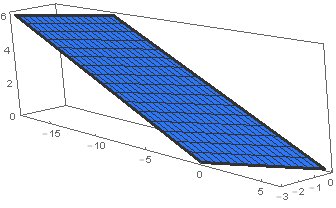
\includegraphics[width=1\linewidth]{../Imágenes/plano}
					\caption{Plano}
					\label{fig:plano}
				\end{figure}
			\end{column}%
			\hfill%
			\begin{column}{.33\textwidth}
				\begin{figure}
					\centering
					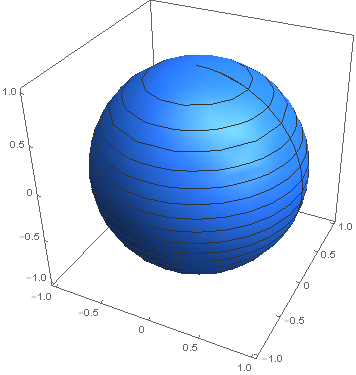
\includegraphics[width=0.8\linewidth]{../Imágenes/esfera}
					\caption{Esfera}
					\label{fig:esfera}
				\end{figure}
			\end{column}%
			\hfill%
			\begin{column}{.33\textwidth}
				\begin{figure}
					\centering
					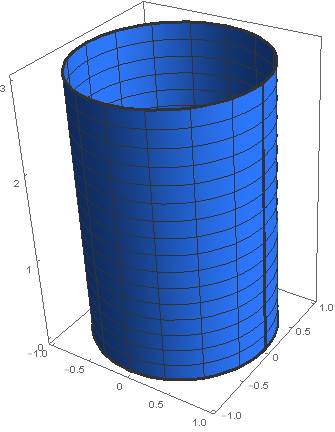
\includegraphics[width=0.7\linewidth]{../Imágenes/cilindro}
					\caption{Cilindro}
					\label{fig:cilindro}
				\end{figure}
			\end{column}%
		\end{columns}

	\end{frame}
	
	\begin{frame}{Introducción}
		\begin{defi}
			Una superficie reglada es aquella generada por una recta en el espacio llamada generatriz, a lo largo de una curva llamada directriz.
		\end{defi}	
		
		\begin{defi}
			Una superficie es reglada si es generada por una familia uniparamétrica de rectas (llamadas generatrices).\\
			
			La parametrización de una superficie reglada es 
			
			\begin{equation}
			r(u,v) = \rho(u) + v a(u)
			\end{equation}
			
			donde $\rho, a : I = [a,b] \to \R^3$ son dos curvas en el espacio.
		\end{defi}
		
		\begin{defi}
			Un conjunto de curvas de una superficie reglada que interseca a cada generatriz en un punto se llama curva generatriz.
		\end{defi}	
		
	\end{frame}
	
	\begin{frame}{Introducción}
		\begin{defi}
			Una superficie reglada es cilíndrica si es de la forma 
			
			\begin{equation}
			r(u,v) = \rho(u) + v a_0
			\end{equation}
			
			con $a_0 \in \R^3$.
		\end{defi}
		
		\begin{defi}
			Una superficie reglada es cónica si es de la forma 
			
			\begin{equation}
			r(u,v) = \rho_0 + v a(u)
			\end{equation}
			
			con $\rho_0 \in \R^3$.\\
			
			$\rho_0$ es el vértice del cono.
		\end{defi}
	\end{frame}
	
	\begin{frame}{Introducción}
			\begin{defi}
				Una superficie reglada es tangente desarrollable si es de la forma 
				
				\begin{equation}
				r(u,v) = \rho(u) + v \rho'(u)
				\end{equation}
			\end{defi}
			
			\begin{defi}
				Una superficie reglada que cumple que $a(u) \neq 0 \ \ \forall u \in I$ se denomina no cilíndrica. 
			\end{defi}
			
			\begin{defi}
				Una superficie no cilíndrica cuyas generatrices son paralelas a un plano directriz fijo se llama superficie de Catalan.
			\end{defi}
			
	\end{frame}
	
	\begin{frame}{Introducción}
		\begin{teo}[Caracterización de las superficies de Catalan]
			Una superficie reglada $r(u,v) = \rho(u) + v a(u)$ es una superficie de Catalan si y sólo si
			\begin{equation}
			[a(u), a'(a), a''(u)] = 0  \ \ \forall u \in I
			\end{equation}.
		\end{teo}
		
		\begin{defi}
			Una superfie de Catalan se dice conoide si todas las generatrices intersecan una recta constante (el eje del conoide).
		\end{defi}
		
	
	\end{frame}
	
	\section{Algunas superficies regladas}
	
	\begin{frame}
		\begin{center}
			\Huge\textbf{\textsf{\textcolor{blue}{Algunas \\ superficies regladas}}}
		\end{center}
	\end{frame}
	
	\subsection{Superficie cilíndrica}
	
	\begin{frame}{Superficie cilíndrica}
		
		\begin{columns}[t] % align columns
			\begin{column}{.60\textwidth}
				\begin{figure}
					\centering
					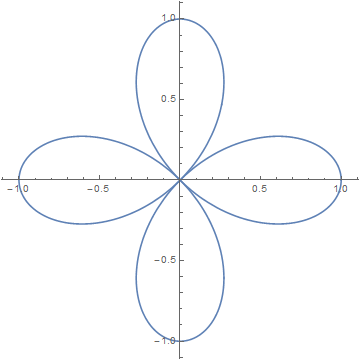
\includegraphics[width=0.8\linewidth]{../Imágenes/rosa-4-petalos}
					\caption{Rosa de cuatro pétalos}
					\label{fig:rosa-4-petalos}
				\end{figure}
			\end{column}%
			\hfill%
			\begin{column}{.40\textwidth}
				$$\begin{array}{rcll}
					a : & [0, 2\pi] & \to & \R^2\\
						& t & \mapsto & (x(t), y(t))
				\end{array}$$
				
			donde 
			
			$$ \begin{cases}
			x(t) = \cos(2t)\cos t \\
			y(t) = \cos(2t) \sen t
			\end{cases} $$
			\end{column}%
		\end{columns}
	
	\end{frame}
	
	\begin{frame}{Superficie cilíndrica}
		
		\begin{columns}[t] % align columns
			\begin{column}{.50\textwidth}
				\begin{figure}
					\centering
					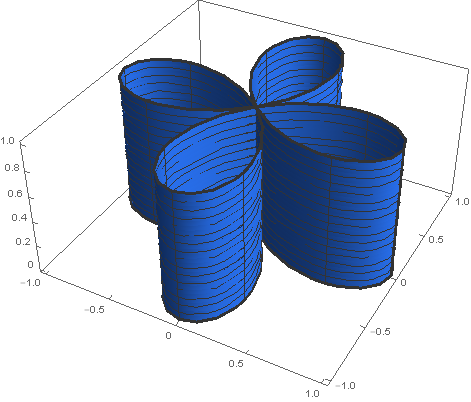
\includegraphics[width=0.8\linewidth]{../Imágenes/cilindro-rosa-4-petalos}
					\caption{Superficie cilíndrica a partir de la rosa de cuatro pétalos}
					\label{fig:cilindro-rosa-4-petalos}
				\end{figure}
			\end{column}%
			\hfill%
			\begin{column}{.50\textwidth}
				$$\begin{array}{rcll}
				r : & [0, 2\pi] \times [0,1] & \to & \R^3\\
				& (u,v) & \mapsto & (x,y,z)
				\end{array}$$
				
				donde 
				
				$$ \begin{cases}
				x(u,v) = \cos(2u)\cos u \\
				y(u,v) = \cos(2u) \sen u \\
				z(u,v) = v
				\end{cases} $$
			\end{column}%
		\end{columns}
		
	\end{frame}
	
	\subsection{Superficie cónica}
	
	\begin{frame}{Superficie cónica}
		\begin{columns}[t] % align columns
			\begin{column}{.50\textwidth}
				\begin{figure}
					\centering
					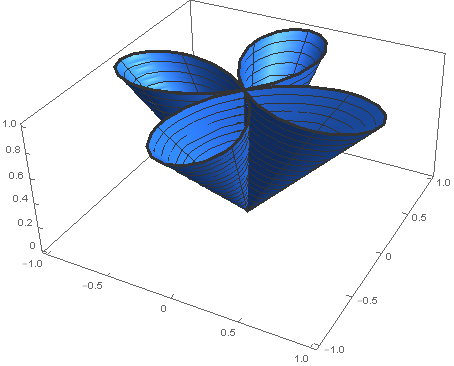
\includegraphics[width=0.8\linewidth]{../Imágenes/cono-rosa-4-petalos}
					\caption{Superficie cónica a partir de la rosa de cuatro pétalos}
					\label{fig:cono-rosa-4-petalos}
				\end{figure}
			\end{column}%
			\hfill%
			\begin{column}{.50\textwidth}
				$$\begin{array}{rcll}
				r : & [0, 2\pi] \times [0,1] & \to & \R^3\\
				& (u,v) & \mapsto & (x,y,z)
				\end{array}$$
				
				donde 
				
				$$ \begin{cases}
				x(u,v) = v\cos(2u)\cos u \\
				y(u,v) = v\cos(2u) \sen u \\
				z(u,v) = v
				\end{cases} $$
			\end{column}%
		\end{columns}
	\end{frame}
	
	\subsection{Conoides}
	
	\subsubsection{Conoide de Wallis}
	
	\begin{frame}{Conoide de Wallis}
		\begin{columns}[t] % align columns
			\begin{column}{.50\textwidth}
				\begin{figure}
					\centering
					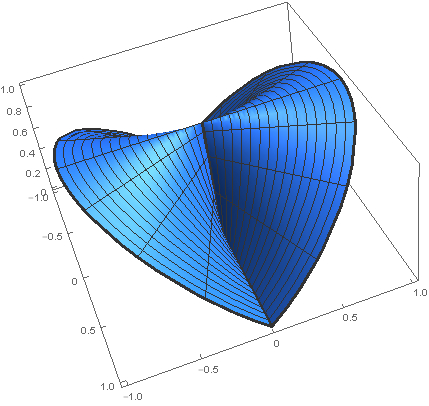
\includegraphics[width=0.8\linewidth]{../Imágenes/conoide-de-Wallis-1}
					\caption{Conoide de Wallis con $a=b=c=1$}
					\label{fig:conoide-de-Wallis-1}
				\end{figure}
			\end{column}%
			\hfill%
			\begin{column}{.50\textwidth}
				$$\begin{array}{rcll}
				r : & [0, 2\pi] \times [0,1] & \to & \R^3\\
				& (u,v) & \mapsto & (x,y,z)
				\end{array}$$
				
				donde 
				
				$$ \begin{cases}
				x(u,v) = v \cos u \\
				y(u,v) = v \sen u \\
				z(u,v) = c \sqrt{a^2 - b^2 \cos^2 u}
				\end{cases} $$
			\end{column}%
		\end{columns}
	\end{frame}
	
	\begin{frame}{Conoide de Wallis}
		\begin{columns}[t] % align columns
			\begin{column}{.50\textwidth}
				\begin{figure}
					\centering
					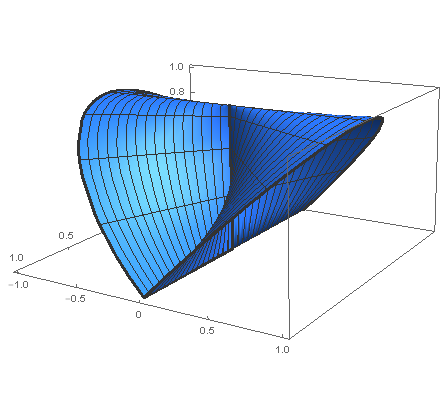
\includegraphics[width=0.8\linewidth]{../Imágenes/conoide-de-Wallis-2}
					\caption{Otra vista del conoide de Wallis con $a=b=c=1$}
					\label{fig:conoide-de-Wallis-2}
				\end{figure}
			\end{column}%
			\hfill%
			\begin{column}{.50\textwidth}
				\textcolor{red}{Añadir imagen}
				%\begin{figure}
				%	\centering
				%	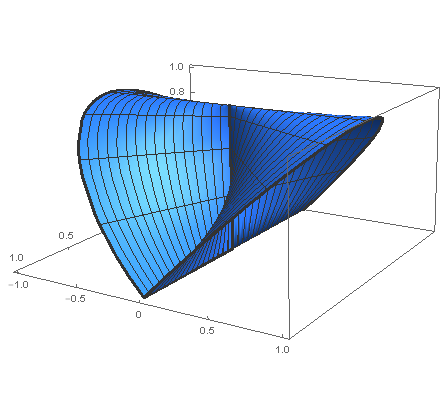
\includegraphics[width=0.8\linewidth]{../Imágenes/conoide-de-Wallis-2}
				%	\caption{Otra vista del conoide de Wallis con $a=b=c=1$}
				%	\label{fig:conoide-de-Wallis-3}
				%\end{figure}
			\end{column}%
		\end{columns}
	\end{frame}
	
	\begin{frame}{Conoide de Wallis}
		\animategraphics[width=4in,height=2in,autoplay,controls,loop]{12}{../Imágenes/Conoide-de-Wallis/Wallis_Conical_Edge-}{0}{59}
	\end{frame}
	
	\subsubsection{Conoide de Plücker}
	
	\begin{frame}{Conoide de Plücker}
		\begin{columns}[t] % align columns
			\begin{column}{.50\textwidth}
				\begin{figure}
					\centering
					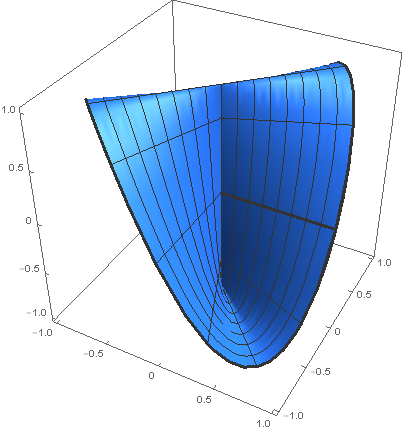
\includegraphics[width=0.8\linewidth]{../Imágenes/conoide-de-Plucker-n=2-1}
					\caption{Conoide de Plücker}
					\label{fig:conoide-de-Plucker-1}
				\end{figure}
			\end{column}%
			\hfill%
			\begin{column}{.50\textwidth}
				$$\begin{array}{rcll}
				r : & [0, 2\pi] \times [0,1] & \to & \R^3\\
				& (u,v) & \mapsto & (x,y,z)
				\end{array}$$
				
				donde 
				
				$$ \begin{cases}
				x(u,v) = v \cos u \\
				y(u,v) = v \sen u \\
				z(u,v) = \sen 2u
				\end{cases} $$
			\end{column}%
		\end{columns}
	\end{frame}
	
	\begin{frame}{Conoide de Plücker}
		\begin{columns}[t] % align columns
			\begin{column}{.50\textwidth}
				\begin{figure}
					\centering
					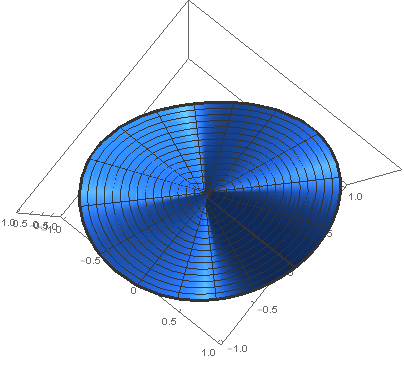
\includegraphics[width=0.8\linewidth]{../Imágenes/conoide-de-Plucker-n=2-2}
					\caption{Otra vista del conoide de Plücker}
					\label{fig:conoide-de-Plücker-2}
				\end{figure}
			\end{column}%
			\hfill%
			\begin{column}{.50\textwidth}
				\textcolor{red}{Añadir imagen}
			\end{column}%
		\end{columns}
	\end{frame}
	
	\begin{frame}{Conoide de Plücker}
		\animategraphics[width=4in,height=2in,autoplay,controls,loop]{12}{../Imágenes/Conoide-de-Plücker(n=2)/Plucker_conoid_(n=2)-}{0}{79}
	\end{frame}
	
	\subsubsection{Conoide de Plücker generalizado}
	
	\begin{frame}{Conoide de Plücker generalizado}
		\begin{columns}[t] % align columns
			\begin{column}{.50\textwidth}
				\begin{figure}
					\centering
					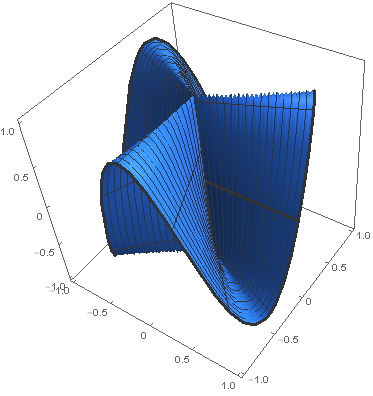
\includegraphics[width=0.8\linewidth]{../Imágenes/conoide-de-Plucker-n=3-1}
					\caption{Conoide de Plücker generalizado con $n=3$}
					\label{fig:conoide-de-Plucker-generalizado-1}
				\end{figure}
			\end{column}%
			\hfill%
			\begin{column}{.50\textwidth}
				$$\begin{array}{rcll}
				r : & [0, 2\pi] \times [0,1] & \to & \R^3\\
				& (u,v) & \mapsto & (x,y,z)
				\end{array}$$
				
				donde 
				
				$$ \begin{cases}
				x(u,v) = v \cos u \\
				y(u,v) = v \sen u \\
				z(u,v) = \sen nu
				\end{cases} $$
			\end{column}%
		\end{columns}
	\end{frame}
	
	\begin{frame}{Conoide de Plücker generalizado}
		\begin{columns}[t] % align columns
			\begin{column}{.50\textwidth}
				\begin{figure}
					\centering
					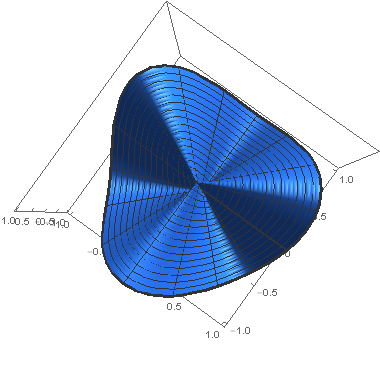
\includegraphics[width=0.8\linewidth]{../Imágenes/conoide-de-Plucker-n=3-2}
					\caption{Otra vista del conoide de Plücker generalizado con $n=3$}
					\label{fig:conoide-de-Plücker-generalizado-2}
				\end{figure}
			\end{column}%
			\hfill%
			\begin{column}{.50\textwidth}
				\textcolor{red}{Añadir imagen}
			\end{column}%
		\end{columns}
	\end{frame}
	
	\begin{frame}{Conoide de Plücker generalizado}
		\animategraphics[width=4in,height=2in,autoplay,controls,loop]{12}{../Imágenes/Conoide-de-Plücker(n=3)/Plucker_conoid_(n=3)-}{0}{79}
	\end{frame}
	
	\subsubsection{Paraguas de Whitney}
	
	\begin{frame}{Paraguas de Whitney}
		\begin{columns}[t] % align columns
			\begin{column}{.50\textwidth}
				\begin{figure}
					\centering
					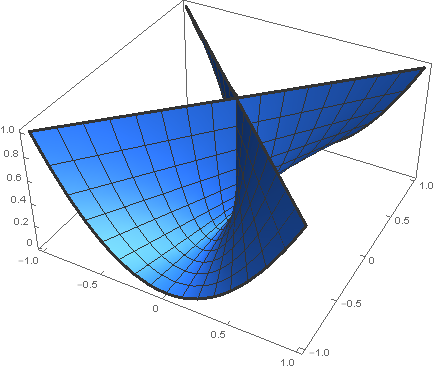
\includegraphics[width=0.8\linewidth]{../Imágenes/paraguas-de-whitney-1}
					\caption{Paraguas de Whitney}
					\label{fig:paraguas-de-Whitney-1}
				\end{figure}
			\end{column}%
			\hfill%
			\begin{column}{.50\textwidth}
				$$\begin{array}{rcll}
				r : & [-1, 1]^2 & \to & \R^3\\
				& (u,v) & \mapsto & (x,y,z)
				\end{array}$$
				
				donde 
				
				$$ \begin{cases}
				x(u,v) = uv \\
				y(u,v) = u \\
				z(u,v) = v^2
				\end{cases} $$
			\end{column}%
		\end{columns}
	\end{frame}
	
	\begin{frame}{Paraguas de Whitney}
		\begin{columns}[t] % align columns
			\begin{column}{.50\textwidth}
				\begin{figure}
					\centering
					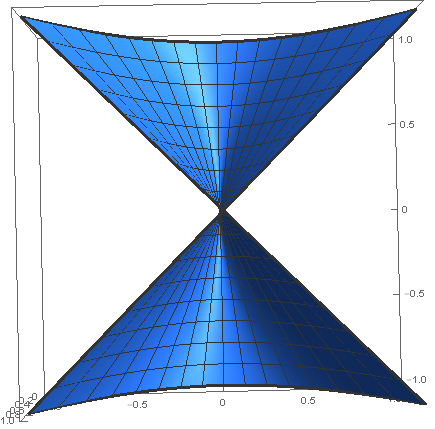
\includegraphics[width=0.8\linewidth]{../Imágenes/paraguas-de-whitney-2}
					\caption{Otra vista del paraguas de Whitney}
					\label{fig:paraguas-de-Whitney-2}
				\end{figure}
			\end{column}%
			\hfill%
			\begin{column}{.50\textwidth}
				\textcolor{red}{Añadir imagen}
			\end{column}%
		\end{columns}
	\end{frame}
	
	\begin{frame}{Paraguas de Whitney}
		\animategraphics[width=4in,height=2in,autoplay,controls,loop]{12}{../Imágenes/Paraguas-de-Whitney/Whitney_umbrella-}{0}{59}
	\end{frame}
	
	\subsection{Otras}
	
	\subsubsection{Banda de Möbius}
	
	\begin{frame}{Banda de Möbius}
		\begin{columns}[t] % align columns
			\begin{column}{.50\textwidth}
				\begin{figure}
					\centering
					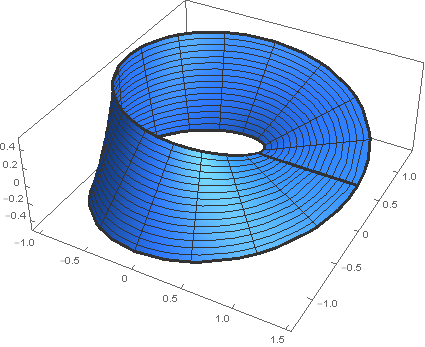
\includegraphics[width=0.8\linewidth]{../Imágenes/banda-de-moebius}
					\caption{Banda de Möbius}
					\label{fig:banda-de-moebius}
				\end{figure}
			\end{column}%
			\hfill%
			\begin{column}{.50\textwidth}
				$$\begin{array}{rcll}
				r : & [0, 2\pi] \times [-1,1] & \to & \R^3\\
				& (u,v) & \mapsto & (x,y,z)
				\end{array}$$
				
				donde 
				
				$$ \begin{cases}
				x(u,v) = \left( 1 + \frac{v}{2}\cos\frac{u}{2} \right)\cos u \\
				y(u,v) = \left( 1 + \frac{v}{2}\cos\frac{u}{2} \right)\sen u \\
				z(u,v) = \frac{v}{2}\sen\frac{u}{2}
				\end{cases} $$
			\end{column}%
		\end{columns}
	\end{frame}
	
	\begin{frame}{Banda de Möbius}
		\animategraphics[width=4in,height=2in,autoplay,controls,loop]{12}{../Imágenes/Banda-de-Moebius/Mobius_strip-}{0}{119}
	\end{frame}
	
	\subsubsection{Helicoide}
	
	\begin{frame}{Helicoide}
		\begin{columns}[t] % align columns
			\begin{column}{.50\textwidth}
				\begin{figure}
					\centering
					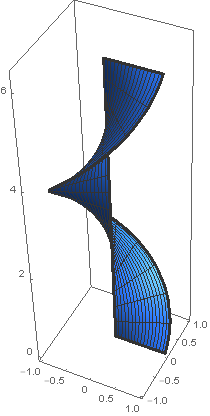
\includegraphics[width=0.5\linewidth]{../Imágenes/helicoide}
					\caption{Helicoide}
					\label{fig:helicoide}
				\end{figure}
			\end{column}%
			\hfill%
			\begin{column}{.50\textwidth}
				$$\begin{array}{rcll}
				r : & [0, 2\pi] \times \R & \to & \R^3\\
				& (u,v) & \mapsto & (x,y,z)
				\end{array}$$
				
				donde 
				
				$$ \begin{cases}
				x(u,v) = v\cos u \\
				y(u,v) = v\sen u \\
				z(u,v) = u
				\end{cases} $$
			\end{column}%
		\end{columns}
	\end{frame}
	
	\begin{frame}{Helicoide}
		\animategraphics[width=4in,height=2in,autoplay,controls,loop]{12}{../Imágenes/Helicoide/helicoid-}{0}{79}
	\end{frame}
	
	\subsubsection{Hiperboloide}
	
	\begin{frame}{Hiperboloide}
		\begin{columns}[t] % align columns
			\begin{column}{.50\textwidth}
				\begin{figure}
					\centering
					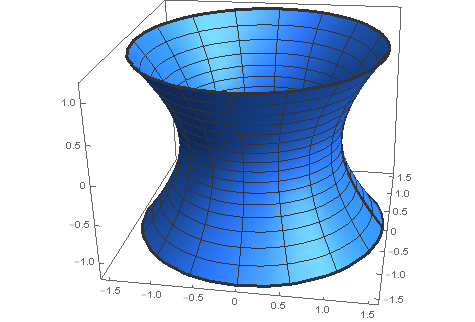
\includegraphics[width=0.9\linewidth]{../Imágenes/hiperboloide}
					\caption{Hiperboloide con $a=b=c=1$}
					\label{fig:hiperboloide}
				\end{figure}
			\end{column}%
			\hfill%
			\begin{column}{.50\textwidth}
				$$\begin{array}{rcll}
				r : & \R \times [0, 2\pi] & \to & \R^3\\
				& (u,v) & \mapsto & (x,y,z)
				\end{array}$$
				
				donde 
				
				$$ \begin{cases}
				x(u,v) = a \cosh u \cos v \\
				y(u,v) = b \cosh u \sen v \\
				z(u,v) = c \senh u
				\end{cases} $$
			\end{column}%
		\end{columns}
	\end{frame}
	
	\section{Aplicaciones a la arquitectura}
	
	\begin{frame}
		\begin{center}
			\Huge\textbf{\textsf{\textcolor{blue}{Aplicaciones \\ a la arquitectura}}}
		\end{center}
	\end{frame}

	\begin{frame}{Aplicaciones a la arquitectura}	
		\begin{figure}
			\centering
			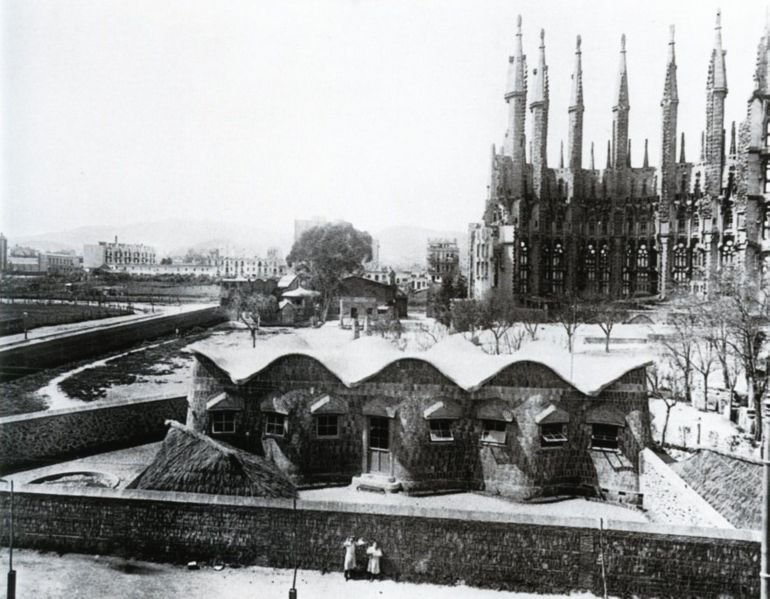
\includegraphics[width=0.5\linewidth]{../Imágenes/Aplicaciones/Escuelas_Sagrada_Familia}
			\caption{Techo de la Escuela de la Sagrada Familia. \url{http://en.wikipedia.org/wiki/File:Escuelas_Sagrada_Familia.jpg}}
			\label{fig:Sagrada-familia}
		\end{figure}	
	\end{frame}
	
	\begin{frame}{Aplicaciones a la arquitectura}	
		\begin{figure}
			\centering
			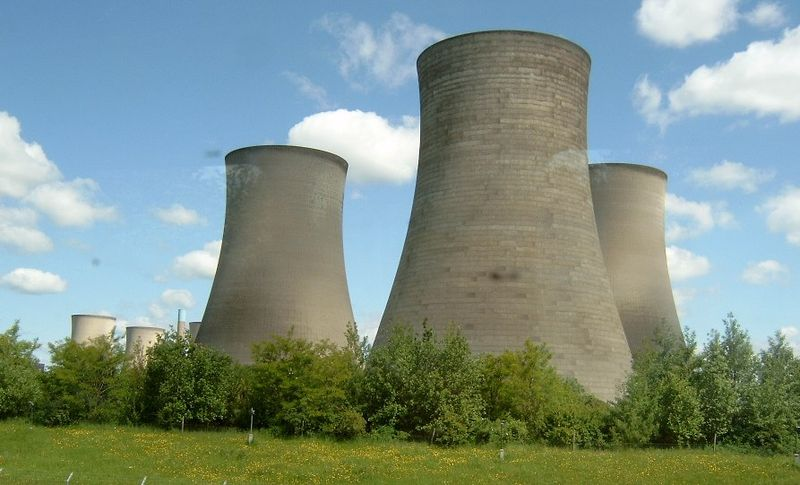
\includegraphics[width=0.8\linewidth]{../Imágenes/Aplicaciones/Didcot_power_station_cooling_tower_zootalures}
			\caption{Torre de refrigeración en Didcot, Reino Unido \url{http://en.wikipedia.org/wiki/File:Didcot_power_station_cooling_tower_zootalures.jpg}}
			\label{fig:Didicot}
		\end{figure}	
	\end{frame}
	
	\begin{frame}{Aplicaciones a la arquitectura}	
		\begin{figure}
			\centering
			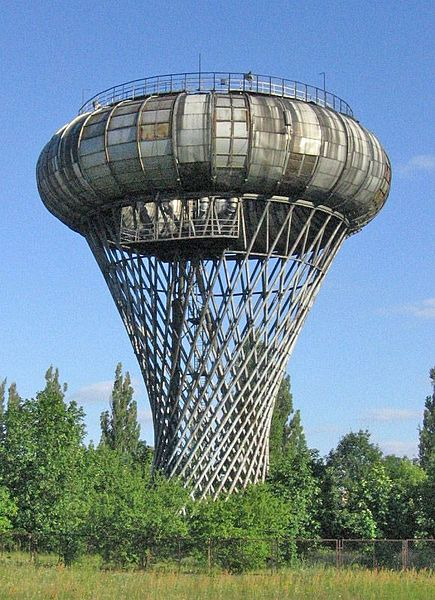
\includegraphics[width=0.4\linewidth]{../Imágenes/Aplicaciones/Ciechanow_water_tower}
			\caption{Torre de agua en Ciechanów, Polonia \url{http://en.wikipedia.org/wiki/File:Ciechanow_water_tower.jpg}}
			\label{fig:torre-agua}
		\end{figure}	
	\end{frame}
	
	\begin{frame}{Aplicaciones a la arquitectura}	
		\begin{figure}
			\centering
			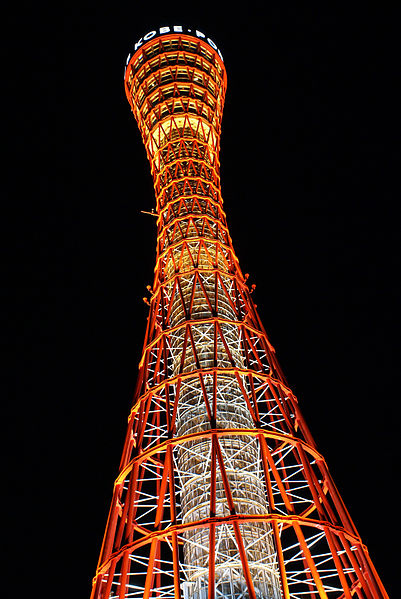
\includegraphics[width=0.35\linewidth]{../Imágenes/Aplicaciones/Kobe_port_tower11s3200}
			\caption{Torre del puerto en Kobe, Japón \url{http://en.wikipedia.org/wiki/File:Kobe_port_tower11s3200.jpg}}
			\label{fig:torre-japon}
		\end{figure}	
	\end{frame}
	
	\begin{frame}{Aplicaciones a la arquitectura}	
		\begin{figure}
			\centering
			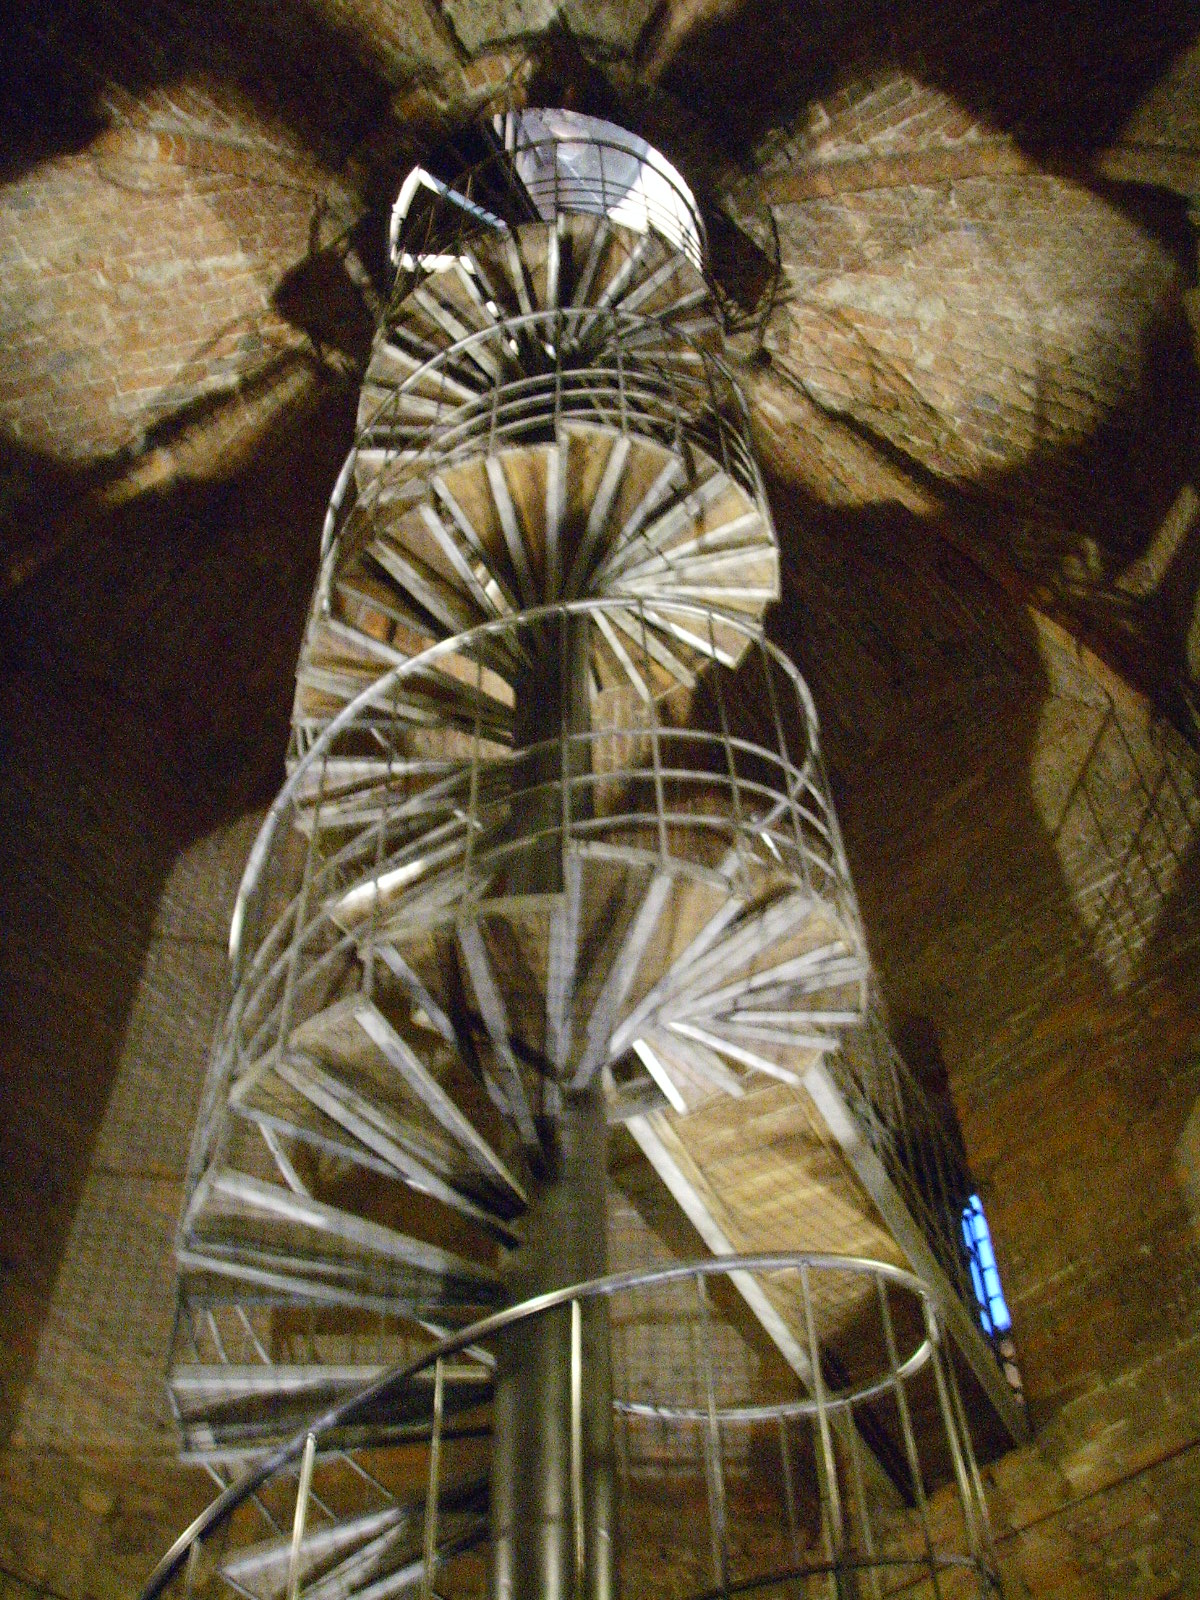
\includegraphics[width=0.35\linewidth]{../Imágenes/Aplicaciones/Cremona,_torrazzo_interno_02_scala_a_chiocciola}
			\caption{Escaleras en el interior de la Torrazzo di Cremona
			\url{http://en.wikipedia.org/wiki/File:Cremona,_torrazzo_interno_02_scala_a_chiocciola.JPG}}
			\label{fig:italia}
		\end{figure}	
	\end{frame}
	
	\begin{frame}{Aplicaciones a la arquitectura}	
		\begin{figure}
			\centering
			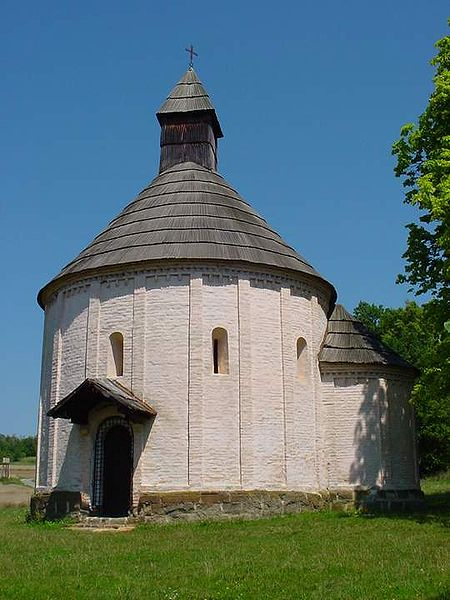
\includegraphics[width=0.35\linewidth]{../Imágenes/Aplicaciones/Nagytotlak}
			\caption{Iglesia en Selo, Eslovenia
			\url{http://en.wikipedia.org/wiki/File:Nagytotlak.JPG}}
			\label{fig:eslovenia}
		\end{figure}	
	\end{frame}
	
	\begin{frame}{Aplicaciones a la arquitectura}	
		\begin{figure}
			\centering
			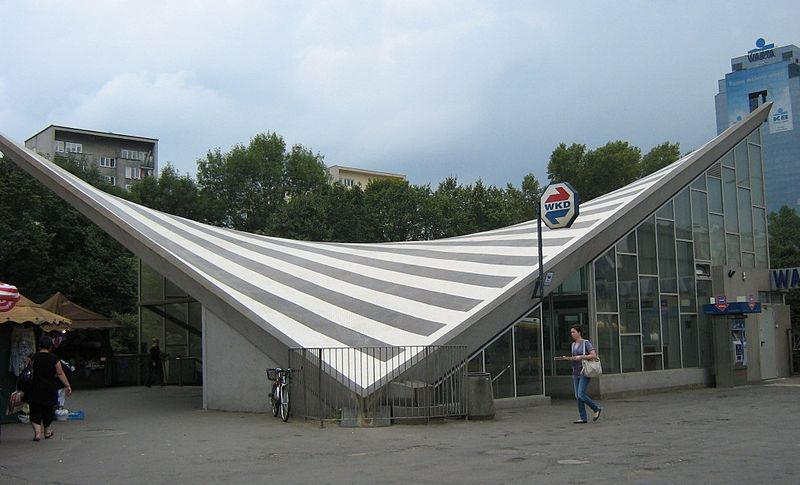
\includegraphics[width=0.6\linewidth]{../Imágenes/Aplicaciones/W-wa_Ochota_PKP-WKD}
			\caption{Techo de la estación de ferrocarriles de Ochota en Varsovia, Polonia
				\url{http://en.wikipedia.org/wiki/File:W-wa_Ochota_PKP-WKD.jpg}}
			\label{fig:trenes}
		\end{figure}	
	\end{frame}
	
\end{document}